
\documentclass{beamer}
\usetheme{Madrid}
\usepackage{graphicx,harvard}
\title{Structure and meaning}
\author{Liam Keeble}
\institute{School of English Literature, Language and Linguistics}
\date{}



\begin{document}


\frame{\titlepage}

\begin{frame}{Introductions}
\begin{itemize}
\item Who am I?
\item What is this module about?
\item How is it going to run?
\end{itemize}
\end{frame}

\begin{frame}{Overview}
\tableofcontents
\end{frame}

\section{What is communication?}

\begin{frame}{What is communication?}
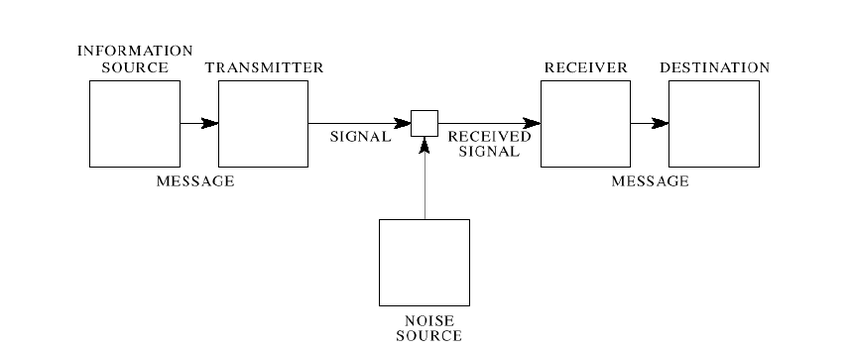
\includegraphics[scale=0.4]{shannon.png}
\nocite{shannon1948mathematical}
\end{frame}


\section{What is language?}

\begin{frame}{Where is language?}
	\begin{itemize}
	\item I-language: the capabilities human beings have to construct linguistic structures
	\item E-language: the externalisation of language (e.g. things that speakers say, also know as utterances)
	\end{itemize}

\end{frame}




\begin{frame}{What is language?}
	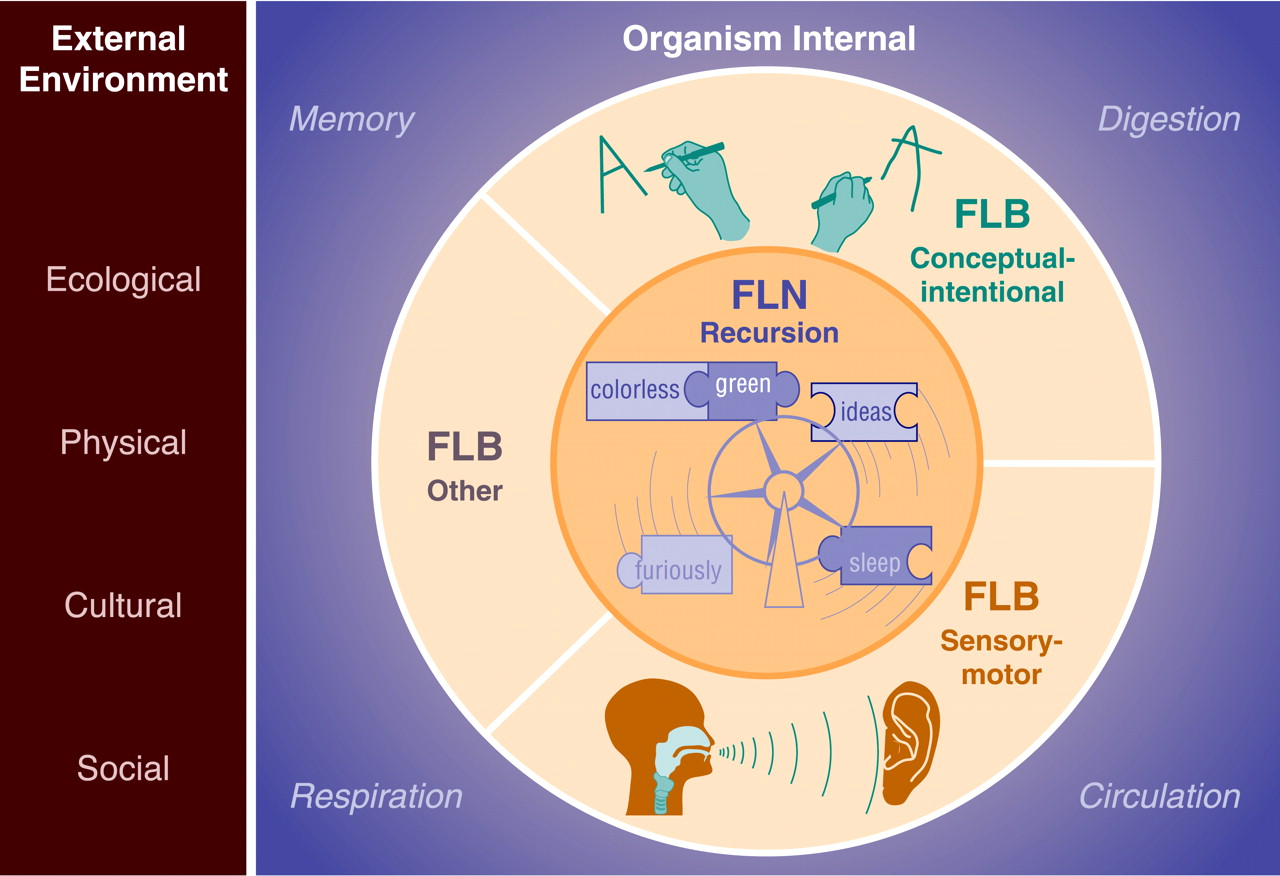
\includegraphics[scale=0.25]{FLN.jpg}
	\nocite{hauser2002faculty}
\end{frame}


\section{Structure in language and meaning}

\begin{frame}{Morphology and meaning}

\end{frame}

\begin{frame}{Syntax and meaning}

\end{frame}



\begin{frame}{References}
\bibliographystyle{agsm}
\bibliography{references.bib}
\end{frame}


\end{document}















